\documentclass[beamer]{BetterDocument}

\addbibresource{ressources.bib}
\beamerBackground{img/background.jpg}

\definecolor{titlecolor}{HTML}{FFFFFF}
\definecolor{titlebg}{HTML}{4db6ac}
\definecolor{sectionBg}{HTML}{26a69a}

\title{Magic Book}
\author{DEROUIN Auréline 21806986\\
	MARTIN Justine 21909920 \\
	THOMAS Maxime 21810751 \\
	STEPANIAK Dimitri 21709178}
\institute{UniCaen}
\date{2019 - 2020}

\begin{document}

	\frame{\titlepage}

	\begin{frame}
		\frametitle{Table des matières}

		\tableofcontents
	\end{frame}

	% Apparait dans le sommaire mais ne met pas le titre de la section sur la diapo (en haut à gauche)
	\section{Présentation d'un LDVH}
	\section{}
	\begin{frame}
		\frametitle{Présentation d'un LDVH}

		\center
\includegraphics[height=0.4\paperheight, keepaspectratio]{img/ldvh1.jpg}\\
		\textit{cf : \cite{book:loupSolitaire}}
	\end{frame}

	\section{Présentation de l'application}
	\subsection{L'interface d'édition}
	\begin{frame}
		\frametitle{Fenêtre principale}

		\center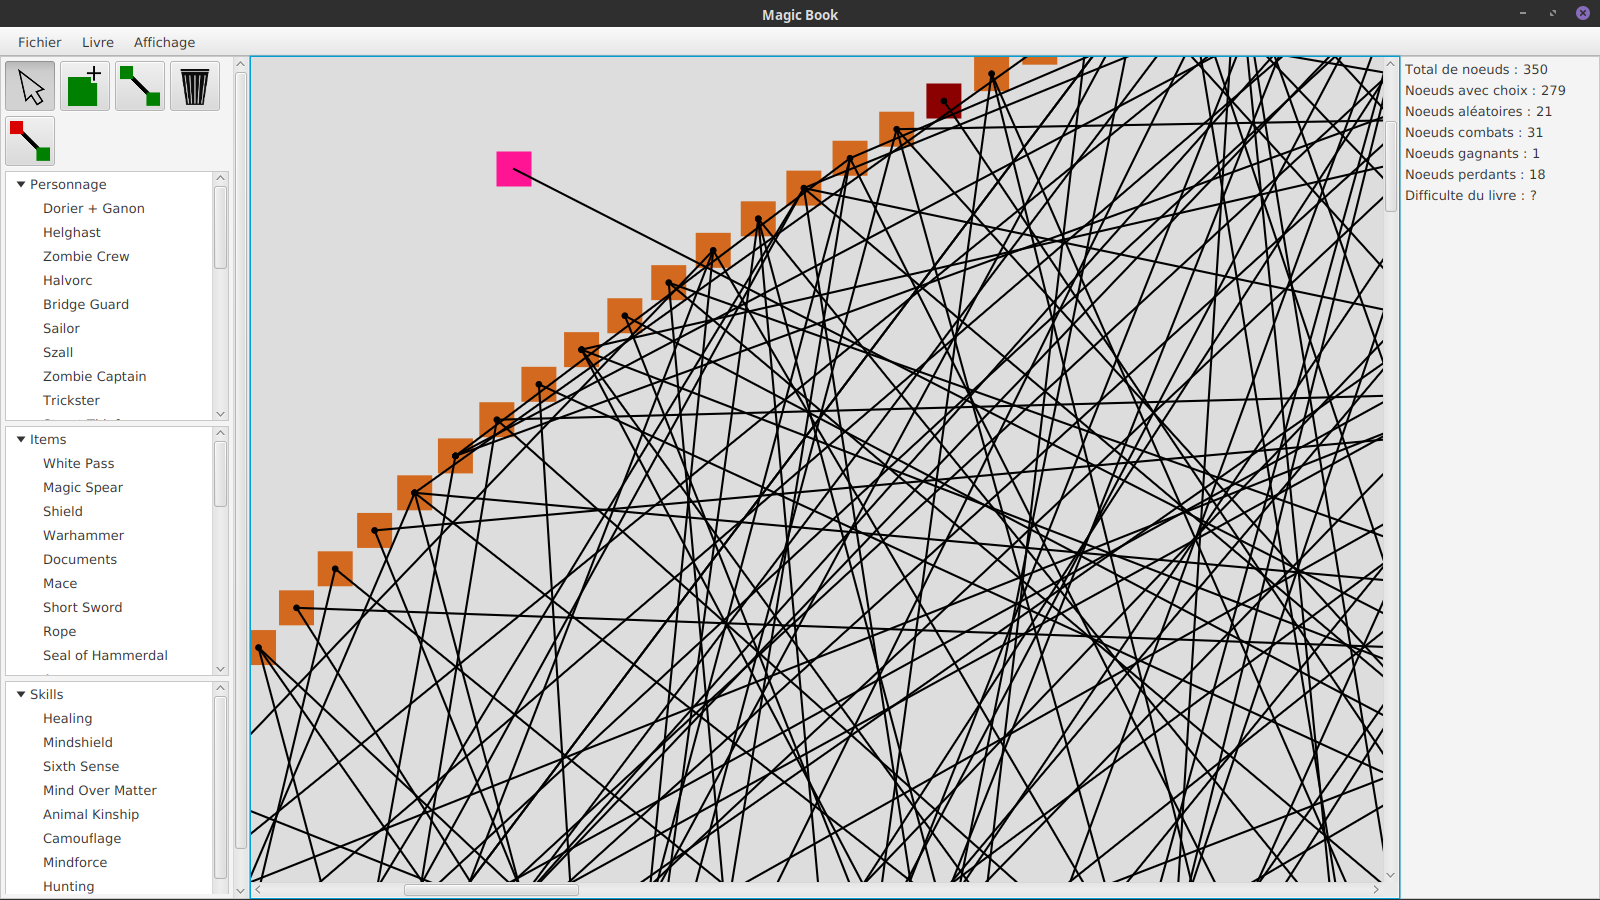
\includegraphics[width=0.8\paperwidth, keepaspectratio]{img/editeur.png}
	\end{frame}

	\begin{frame}
		\frametitle{Exemple de boîte de dialogue}

		\center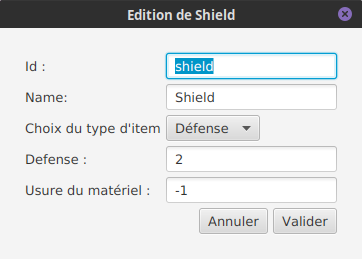
\includegraphics[width=0.4\paperwidth, keepaspectratio]{img/editeur_item.png}
	\end{frame}

	\subsection{L'interface de jeu}
	\begin{frame}
		\frametitle{Paragraphe à choix}

		\center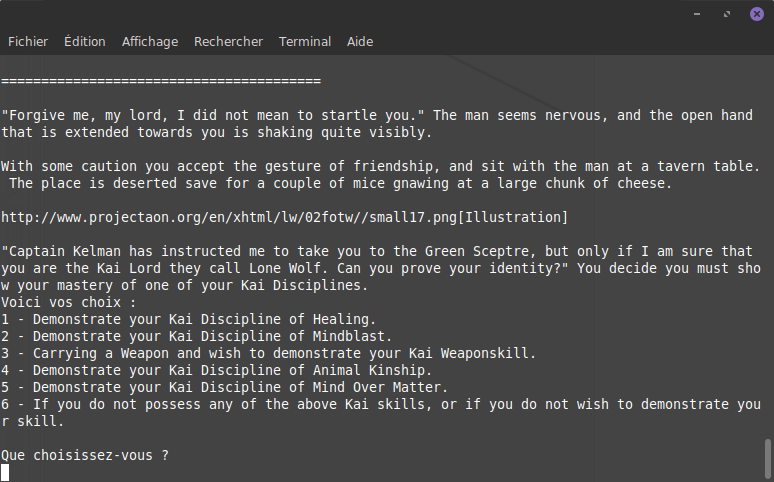
\includegraphics[width=0.8\paperwidth, keepaspectratio]{img/jeu_choix.png}
	\end{frame}

	\begin{frame}
		\frametitle{Paragraphe de combat}

		\center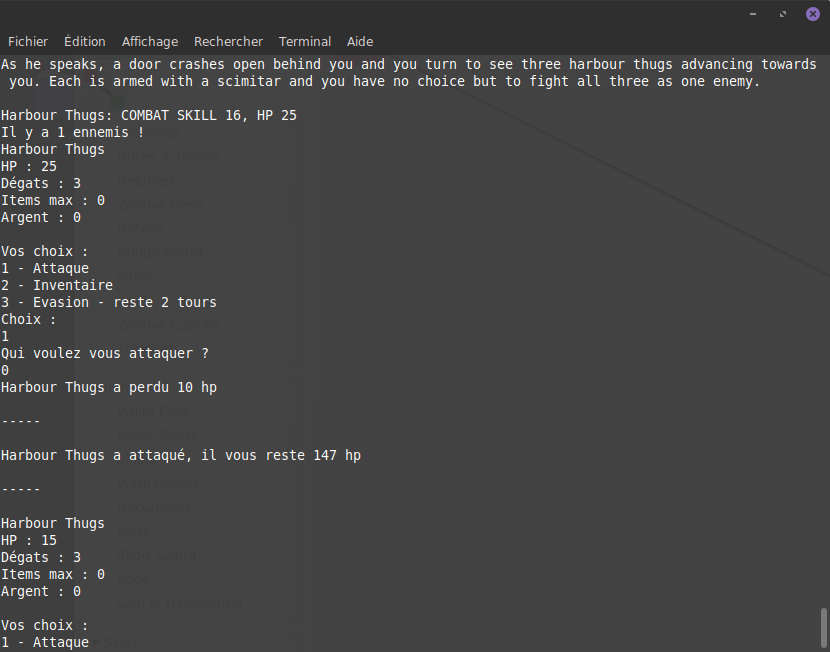
\includegraphics[width=0.7\paperwidth, keepaspectratio]{img/jeu_combat.png}
	\end{frame}

	\section{Estimation de la difficulté d'un livre}
	\subsection{Fonctionnement}
	\begin{frame}
		\frametitle{L'idée d'origine}

		\begin{algorithm}[H]
			\caption{estimer(n, noeudDepart): float}
  			\scriptsize
			\DontPrintSemicolon
			victoire $\gets$ 0\;

			\For{i allant de 0 à n-1}{
				noeudEnCours $\gets$ noeudDepart\;
				\While{noeudEnCours.getStatus() != VICTORY \&\& noeudEnCours.getStatus() != FAILURE}{
					Random rand : Random\;
					nChoix $\gets$ noeudEnCours.getChoices().size()\;
					noeudEnCours = noeudEnCours.getChoices().get(rand.nextInt(nChoix))\;
				}
				\;
				\uIf{nodeTerminal.getStatus() == BookNodeStatus.VICTORY}{
					victoire $\gets$ victoire + 1\;
				}
			}
			\;
			\Return{(100*victoire)/n}
		\end{algorithm}
	\end{frame}

	\begin{frame}
		\frametitle{Les améliorations apportées}

		\center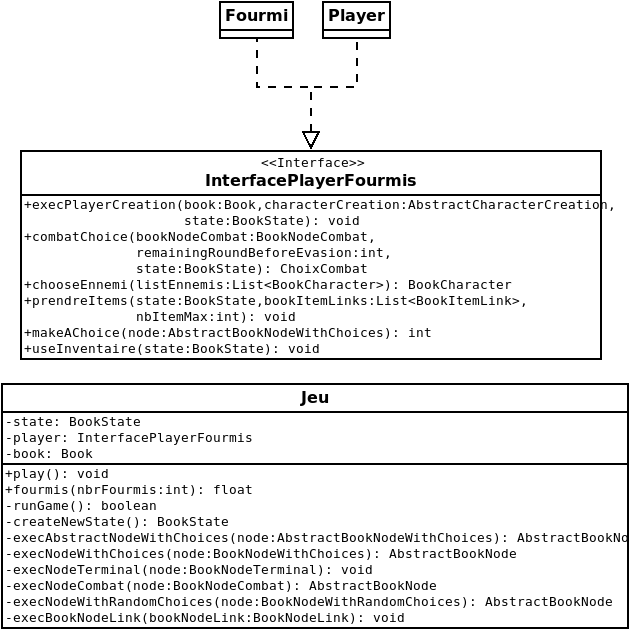
\includegraphics[height=0.7\paperheight, keepaspectratio]{img/FourmisAmelio.png}
	\end{frame}

	\subsection{Problèmes et idées d'amélioration}
	\begin{frame}
		\frametitle{Les points noirs actuels}

		\begin{itemize}
			\item{Code en commun concernant la sélection des items}
			\item{Pas de gestion des shops}
			\item{Pas de durabilité pour les items}
			\item{L'IA achète et prends les items de manière aléatoire}
			\item{Aucune verification n'est faite sur le livre avant d'y jouer}
			\item{L'IA n'est pas efficace lors d'un combat}
		\end{itemize}
	\end{frame}

	\begin{frame}
		\frametitle{Pistes de réflexions}

		\begin{itemize}
			\item{Code en commun concernant la sélection des items}
			\begin{itemize}
				\item{Retourner l'item à sélectionner}
				\item{Gérer l'item retourné}
			\end{itemize}

			\item{Pas de gestion des shops / Pas de durabilité pour les items}
			\begin{itemize}
				\item{Implémenter la fonctionnalité}
			\end{itemize}

			\item{L'IA achète et prends les items de manière aléatoire}
			\begin{itemize}
				\item{Ajouter un champs de "viabilité"}
				\item{Déterminer la rareté et l'importance d'un item}
			\end{itemize}

			\item{Aucune verification n'est faite sur le livre avant d'y jouer}
			\begin{itemize}
				\item{Vérifier le livre}
				\item{Détection de boucle infini}
			\end{itemize}

			\item{L'IA n'est pas efficace lors d'un combat}
			\begin{itemize}
				\item{Optimiser l'utilisation des potions}
				\item{Toujours sélectionner la meilleure arme et armure}
				\item{Déterminer quel est l'ennemi à privilégier}
				\item{Comment gérer l'évasion ?}
			\end{itemize}
		\end{itemize}
	\end{frame}

	\section{Export du livre au format texte}
	\subsection{Mélange des noeuds du livre}
	\begin{frame}
		\frametitle{Exemple d'export d'un livre}

		\center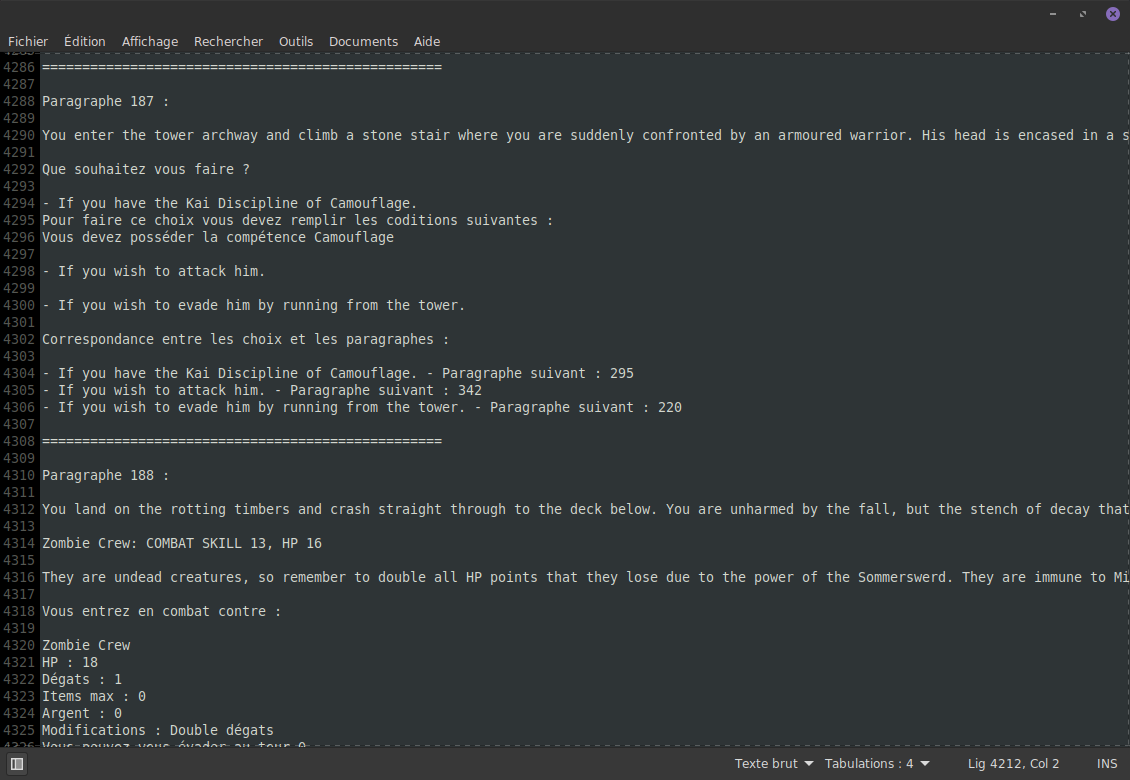
\includegraphics[width=0.8\paperwidth, keepaspectratio]{img/export_txt.png}
	\end{frame}

	\begin{frame}
		\frametitle{Algorithme de mélange}

		\begin{algorithm}[H]
			\caption{melanger(nodes): map<int, AbstractBookNode>}
			\scriptsize
			\DontPrintSemicolon

			shuffle : map<int, AbstractBookNode>\;
			leftNumber : int[1..nodes.length-1]\;
			postNodes : AbstractBookNode[]\;
			rand : Random\;
			\;
			\For{entry<int, AbstractBookNode> e : nodes.entrySet()}{
				\uIf{e.getKey() == 1}{
					shuffle[1] = e.getValue()\;
					continue\;
				} \uElseIf{e.getValue() instanceof BookNodeTerminal}{
					bookNodeTerminal : BookNodeTerminal
					bookNodeTerminal = (BookNodeTerminal) e.getValue()\;
					\uIf{bookNodeTerminal.getBookNodeStatus() == BookNodeStatus.VICTORY}{
						shuffle[leftNumber[leftNumber.length - 1] + 1] = bookNodeTerminal\;
						leftNumber.remove(leftNumber.length - 1)\;
						continue\;
					}
				}

				postNodes.add(e.getValue())\;
			}
		\end{algorithm}
	\end{frame}

	\begin{frame}
		\frametitle{Algorithme de mélange (suite)}

		\begin{algorithm}[H]
			\scriptsize
			\DontPrintSemicolon

			\For{AbstractBookNode bookNode : postNodes}{
				int index = rand.nextInt(leftNumber.size())\;
				shuffle[leftNumber.get(index)+1] = bookNode\;
				leftNumber.remove(index)\;
			}

			\Return{shuffle}\;
		\end{algorithm}
	\end{frame}

	\subsection{Décrire les éléments du livre}
	\begin{frame}
		\frametitle{L'interface \textbf{Descriptible}}

		\center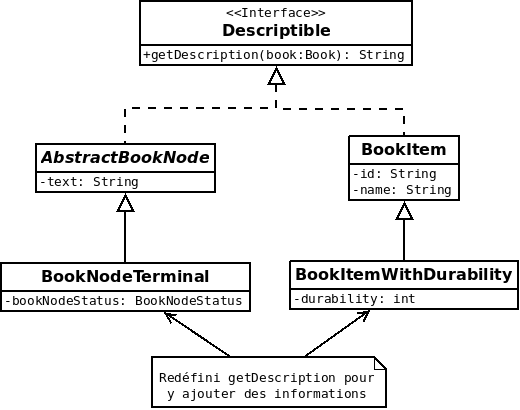
\includegraphics[height=0.7\paperheight, keepaspectratio]{img/descriptible.png}
	\end{frame}

	\begin{frame}[fragile]
		\frametitle{Algorithme d'écriture}

		\begin{lstlisting}[gobble=12, language=java,
    basicstyle=\ttfamily\fontsize{7}{9}\selectfont]
			FileWriter fileWritter = new FileWriter(path);

			fileWritter.write(book.getTextPrelude());
			fileWritter.write("\n");

			writeSeparator(fileWritter);

			for(int i = 0 ; i < book.getCharacterCreations().size() ; i++) {
				fileWritter.write(book.getCharacterCreations().get(i).getDescription(book));
				writeSeparator(fileWritter);
			}

			writeSeparator(fileWritter);

			for(int i = 0 ; i < nodes.size() ; i++) {
				writeNode(nodes.get(i+1), nodesInv, book, fileWritter);
				writeSeparator(fileWritter);
			}
		\end{lstlisting}
	\end{frame}

	\begin{frame}[fragile]
		\frametitle{Algorithme d'écriture}

		\begin{lstlisting}[gobble=12, language=java,
    basicstyle=\ttfamily\fontsize{7}{9}\selectfont]
			private static void writeNode(AbstractBookNode node, HashMap<AbstractBookNode, Integer> nodesIndex, Book book, FileWriter out) throws IOException {
				out.write("Paragraphe " + nodesIndex.get(node) + " :\n");
				out.write("\n");

				out.write(node.getDescription(book));

				if(!node.getChoices().isEmpty()) {
					out.write("\nCorrespondance entre les choix et les paragraphes : \n\n");

					for(BookNodeLink nodeLink : node.getChoices()) {
						out.write("- ");
						out.write(nodeLink.getText());
						out.write(" ");
						out.write("- Paragraphe suivant : ");
						out.write(""+nodesIndex.get(book.getNodes().get(nodeLink.getDestination())));
						out.write("\n");
					}
				}
			}
		\end{lstlisting}
	\end{frame}

	\section{}
	\subsection{}
	\begin{frame}[allowframebreaks]
	  \frametitle{Références}

	  \printbibliography
	 \end{frame}

\end{document}
